% !TEX root = ../rawlik-phd-thesis.tex
\chapter{Axion analysis}
\label{ch:axion-analysis}
In the previous chapter a methodology for searching for oscillations in an unevenly sampled time series was introduced.
Here it is described how it was applied to look for oscillations in the neutron EDM data taken at PSI in the years 2015--17.

First, the scalar coupling of axions to gluons was considered, acting like an oscillating nEDM signal.
The time series of $R$, the ratio of the spin-precession frequency of stored neutrons and ${}^{199}$Hg atoms, was analysed.
No significant signal was found, which allowed the first laboratory limits on the axion coupling to gluons to be put.
This analysis was a joint effort with Nicholas Ayres, who analysed the data of the Grenoble-based nEDM measurement in search for the scalar coupling~\cite{AyresThesis}.
Rather than the raw $R$ time series, he considered nEDM estimates as obtained on a run basis.
The two analyses were complementary, each covering a different range of oscillation frequencies.

An analysis of the derivative coupling of axions to nucleons, acting like on oscillating magnetic field, was also performed.
No significant discovery could be claimed, which led to an improvement upon previous laboratory limits.

Finally, a dedicated method to search for an oscillating nEDM is proposed, which could extend the sensitivity to frequencies up to hundreds of hertz.

% Finally, a particular frequency of \num{23.934}~hours, the sidereal frequency, was considered.
% \marginpar{The sidereal frequency is wthe one of the Earth spinning in the celestial coordinates.}
% Oscillations of that periodicity can be interpreted a hint of a \emph{cosmic spin anisotropy field}~\cite{Altarev2009}.




\section{The PSI 2015--16 data set}
Let us shortly recapitulate the principle of the measurement (discussed in detail in Ch.\,\ref{ch:nedm-at-psi-apparatus}).
The main purpose of the nEDM experiment at PSI was to measure the static neutron electric dipole moment.
To that purpose $R = \nu_\text{n} / \nu_\text{Hg}$, the ratio of spin-precession frequencies of neutrons and ${}^{199}$Hg atoms, was measured in a combination of a magnetic and an electric field.
A non-zero static nEDM would induce an electric-field-dependent shift in the spin-precession frequency of neutrons, and thereby in $R$, too.
In a zero electric field there would be no shift, while the parallel and antiparallel configurations of the magnetic and electric fields would shift $R$ in opposite directions.
\marginpar{In the PSI experiment the electric field was automatically changed according to a looped pattern: 48 cycles in one polarity, 8 cycles without the field, 48 cycles in the other, 8 without the field.}
The nEDM was estimated based on those shifts.
Due to the data blinding,
% \footnote{In order to reduce bias the data were modified upon being taken in a way, that a secret nEDM was injected into them. This additional offset is only revealed as the very last step, once the measurement and analysis have been completed. The data were still blinded at the time of writing.}
a constant shift corresponding to an nEDM of order \SI{e-25}{\elementarycharge\centi\meter} was expected.
Using $R$, that is normalising the precession frequency of neutrons to the one of ${}^{199}$Hg atoms, suppressed the effect of homogeneous variations in the magnetic field.
Even though the neutrons and ${}^{199}$Hg atoms were stored together, the neutrons sagged due to their extremely low speed.
Due to the sag vertical magnetic gradients of the magnetic field caused a shift in $R$.
In order to correct for that effect the vertical gradient was modulated on a sequence basis (several hundred cycles).

% The data used in the analysis were collected at PSI between 2015--07--03, 14:21:30 and 2016--12--18, 19:51:23.
The data used in the analysis were collected at PSI between 2015--07--03 and 2016--12--18.
No measurement dedicated for an oscillating nEDM search was performed.
The time series of $R$, the ratio of the spin-precession frequencies of the neutrons and ${}^{199}$Hg atoms is presented in Fig.\,\ref{fig:PSI_dataset_time_domain}.
\marginpar{A technical term for uninterupted operation was a run.
Sometimes a run was stopped due to technical reasons, and a new started afterwards.
A sequence combines those consecutive runs, that could be one run if not for the interruption.}
Take a look first at the inset in the lower-right corner.
It zooms into data collected within one \emph{sequence}, typically 1--3 days long.
During a sequence the apparatus completed one cycle after another, one every \SI{300}{\second}, each yielding an estimate of $R$.
The electric field was automatically changed between three states: pointing upwards, being zero and pointing downwards.
The different relative orientations of the electric and magnetic fields are depicted in colour in the figure.
Sometimes there were technical breaks in the data taking during a sequence, as in the case of the one shown in the lower-left corner of Fig.\,\ref{fig:PSI_dataset_time_domain}.

\begin{figure}
  \centering
  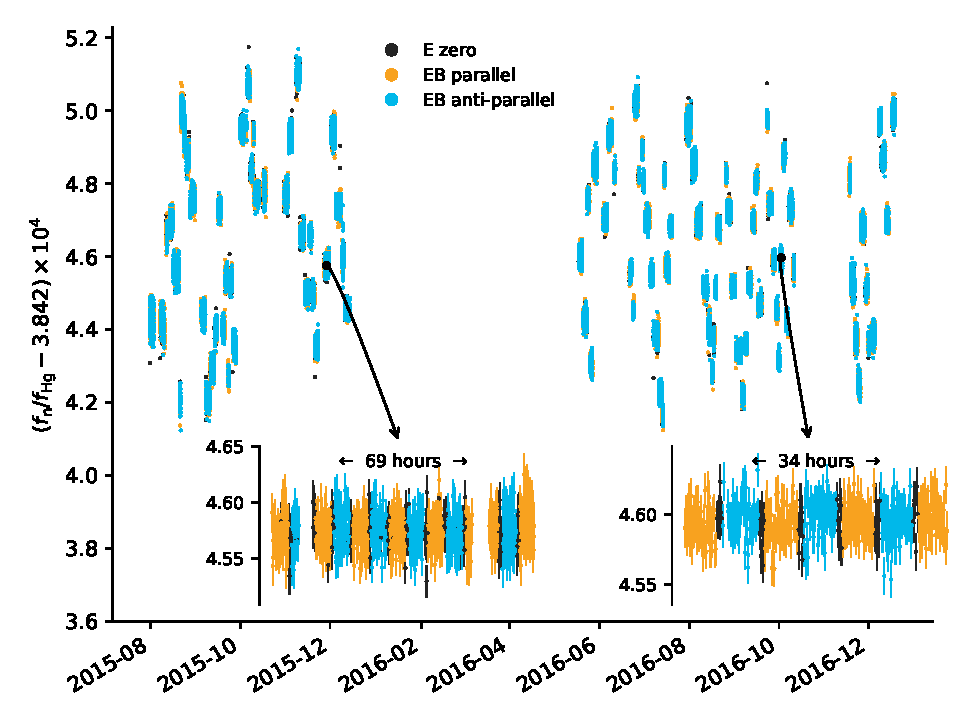
\includegraphics[width=\linewidth]{gfx/axions/deltah4mm_time_domain_inset_no_yerr.pdf}
  \caption{The complete $R = \nu_\text{n} / \nu_\text{Hg}$ time series used in the analysis, measured at PSI between July 2015 and December 2016.
  Two sequences are enlarged (one 69 hours long, the other 34).
  Due to the high density of the measurements individual points cannot be resolved.
  The colours depict the relative orientation of the magnetic and electric fields: $E \uparrow \uparrow B$ (orange), $E \uparrow \downarrow B$ (blue) and $E=0$ (black).
  Between sequences the vertical gradient of the magnetic field was changed, so that those systematic effects, which are linear with the gradient could be interpolated to zero.
  This caused large shifts in $R$.
  The $R$ time series has been corrected for gradient drifts (the correction is relative and does not extend from one sequence to another, for details see text).
  In the insets the points are drawn with their corresponding error bars. See also Fig.\,\ref{fig:oscillating_nEDM_in_R}.}\label{fig:PSI_dataset_time_domain}
\end{figure}

A sequence was taken always in one magnetic field configuration.
In between the sequences the vertical gradient was changed in \SI{10}{\pico\tesla} steps up to $\pm \SI{60}{\pico\tesla}$.
In the static nEDM analysis it allowed for those systematic effects which scale linearly with the gradient to be extrapolated to zero (see Sec.\,\ref{sec:measurement_procedure}).
These large changes in the vertical gradient caused the large shifts in $R$ from one sequence to another.




\section{How a signal would look}
Now we consider how an oscillating electric dipole moment would have affected the $R$ time series, as measured by the PSI experiment.
Should the neutron electric dipole moment oscillate, $R$ would have oscillated as well, even when the electric field was constant.
A reversal of the electric field polarity would have reversed the phase of the oscillations.
With a zero electric field no oscillations would be visible.
In Fig.\,\ref{fig:oscillating_nEDM_in_R} an $R$ time series is depicted, with the combined effect of a large nEDM oscillation and the blinding offset.
Because of the non-zero static nEDM and the phase shift the least-squares spectral analysis could not be applied directly to the $R$ time series.
However, the time series is still a part of a simple harmonic oscillation when only one field configuration is considered.
(We neglect for the moment the inter-sequence shifts.) In the analysis the $R$ time series was split thus into three: a series of points measured without the electric field (not sensitive to an oscillation of the nEDM), one with the electric and magnetic fields parallel and one with antiparallel.
The last two would have the hypothetical oscillation in opposite phases.
We will refer to the three data sets as $E=0$, $E \uparrow \uparrow B$ and $E \uparrow \downarrow B$, respectively.
Each of those was treated separately.

\begin{figure}
  \centering
  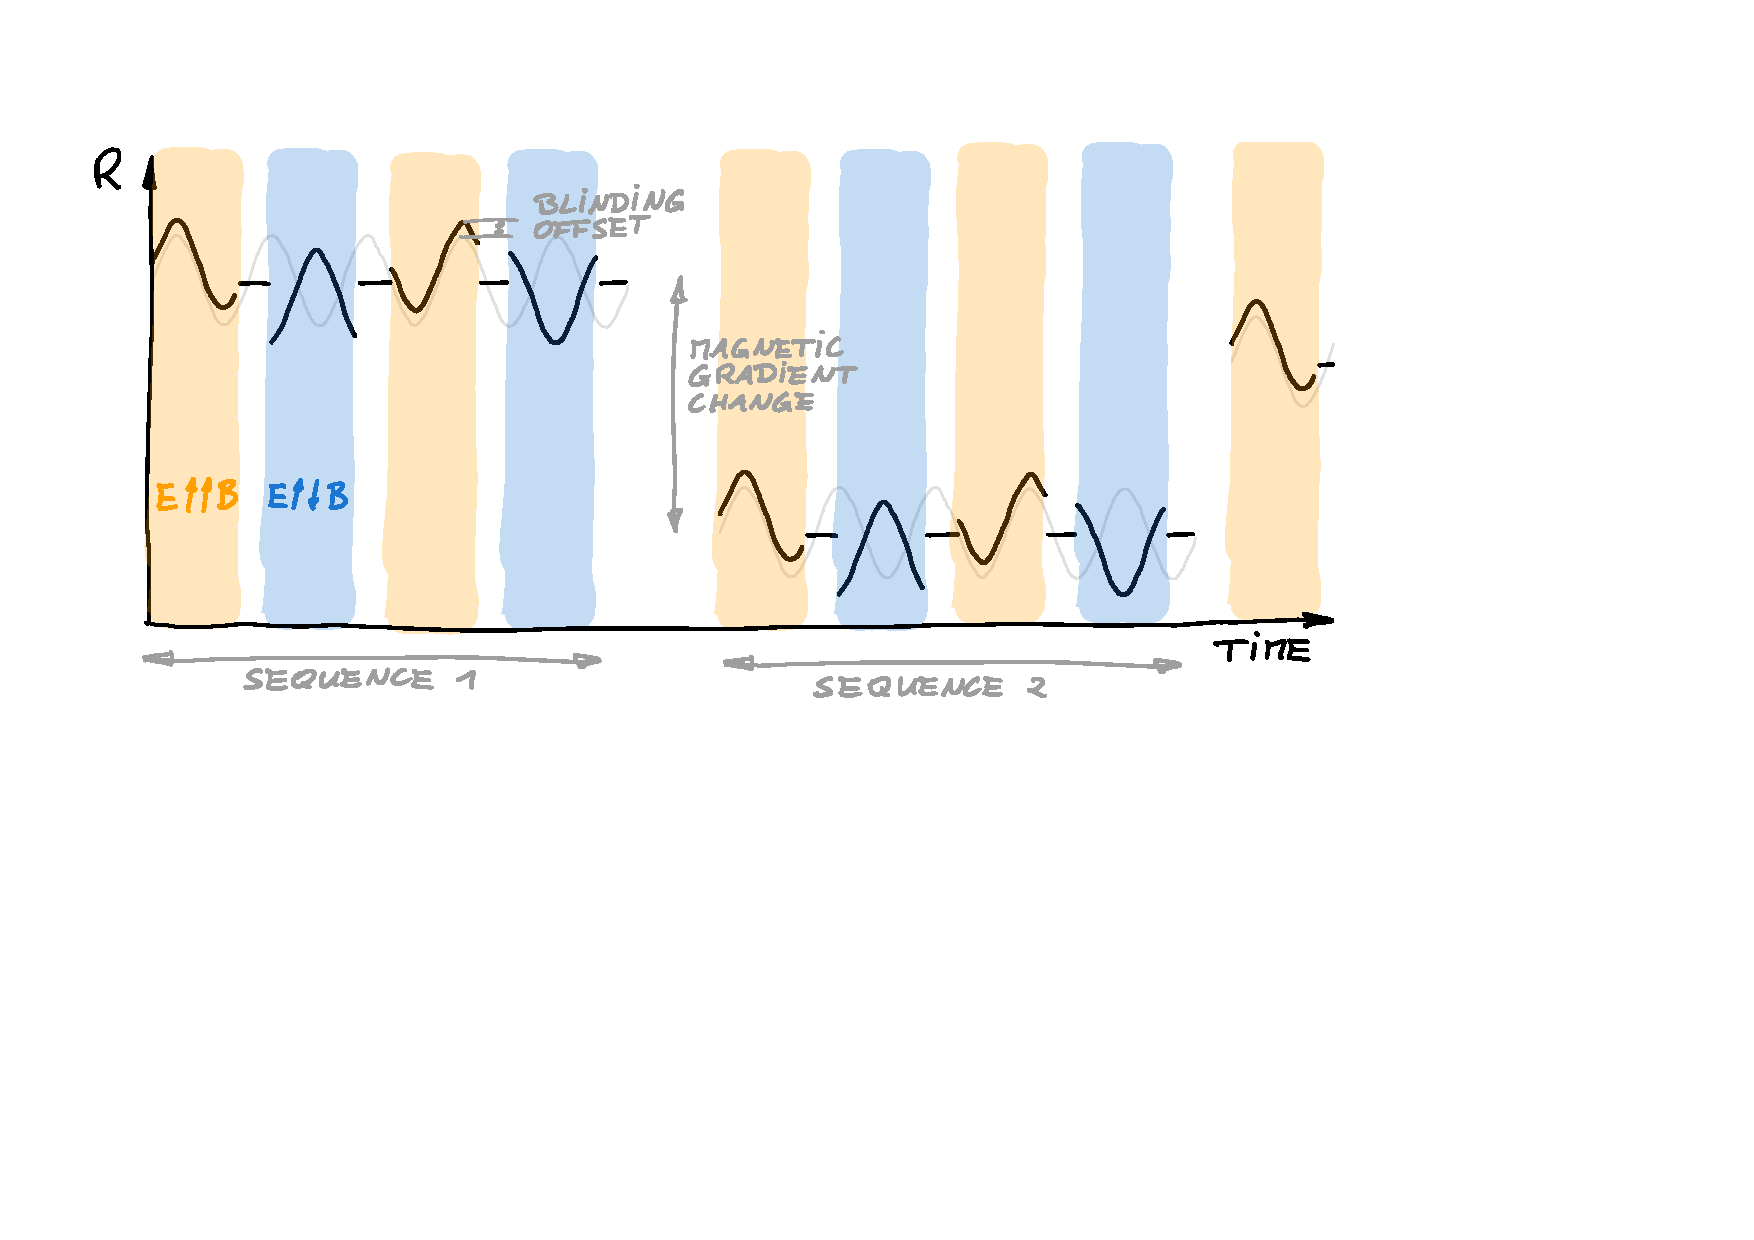
\includegraphics[width=\linewidth]{gfx/axions/signal_illustration.pdf}
  \caption{An illustration of an axion-induced oscillation in the $R = \nu_\text{n} / \nu_\text{Hg}$ time series.
  The colours indicate the configuration of the electric and magnetic fields: parallel to one another ($E \uparrow \uparrow B$, orange) and antiparallel ($E \uparrow \downarrow B$, blue).
  The oscillation in $R$ has an opposite phase in the two configurations.
  The effect of a static nEDM (expected to be large due to the data blinding) is a field-configuration-dependent offset.
  Between sequences the vertical gradient of the magnetic field gradient was changed (so that those systematic effects, which are linear with the gradient could be interpolated to zero). This caused large shifts in $R$.}\label{fig:oscillating_nEDM_in_R}
\end{figure}

A part of the measurement procedure was to deliberately work in a substantial vertical magnetic field gradient.
The gradient changed between sequences, causing large shifts in $R$, as seen in Fig.\,\ref{fig:PSI_dataset_time_domain} and illustrated in Fig.\,\ref{fig:oscillating_nEDM_in_R}.
The problem of inter-sequence jumps was solved by allowing the DC offset in the LSSA fit to be different in each sequence:
\begin{equation}
  \label{eq:axions_LSSA}
  A\sin(2 \pi f t) + B\cos(2 \pi f t) + \sum_i C_i\,\Pi_i(t) \ ,
\end{equation}
where $C_i$ is the free offset in the $i$th sequence and $\Pi_i(t)$ is a gate function equal to one in the $i$th sequence and zero elsewhere.
In this way the model could leverage the coherence of the oscillation across sequences despite the unknown offsets.
The downside was a reduced sensitivity to oscillations slower than a sequence (2--3 days).
These slow oscillations were largely absorbed into the different free offsets.
With this modification the LSSA could be applied to the three data sets in a way as it is described in the previous chapter.

% It may be tempting to think about demodulating the $R$ time-series into what would be expected to be an oscillation. This would require subtracting the DC offset for each electric field configuration, in each run separately, then flipping the signal around the DC level for one configuration. \mnote{The offsets are measured with Cs, mention that.} The disadvantage is that uncertainty in such a demodulation would become a systematic effect and would need to be tightly controlled.

% , as clearly visible in Fig.\,\ref{fig:axions_gradient_drift_correction}.
% The nEDM team spares no effort to measure the gradient. Nevertheless, the achieved precision (\SI[per-mode=symbol]{\approx 1}{\pico\tesla\per\centi\meter}) is only comparable to the one of $f_n$ (in the order of \SI{1}{\pico\tesla}). The exact way how the gradient should determined is highly non--trivial and there is ongoing research in this respect. \mnote{Mention here the exact way the gradient drift correction is done. And cite Elise's thesis.} Actually, even the height difference between the neutrons and $^{199}$Hg centres of mass (a few millimeters) is still discussed. \mnote{Know how exactly was $\Delta h$ determined in the end. Also, mention the definition of a sequence here (as in the paper).}
% \cite{Afach2014magmoment}

% Assuming a constant gradient during a \emph{run} one can determine it much more precise. This assumption, however, is known not to be exactly true.

% One should note, that any, including an oscillating one, nEDM effect affects only the position of the neutrons' resonance. The shape of the resonance curve is unaffected. Therefore, the method to extract neutron Larmor frequency $f_n$, and thereby $R$, for each \emph{cycle} is valid also in case of an oscillating nEDM.




\section{Systematic Effects}
In the analysis the compatibility of the periodogram of the $R$ time series with the one of pure noise, the null hypothesis, was tested.
Variations in $R$ could be considered systematic effects, as they would have resulted in an additional power in the periodogram.

Most prominently, $R$ followed the changes in the vertical gradient of the magnetic field.
The gradient changed not only between the sequences, which was accounted for by modifying the LSSA fit, but also drifted within each sequence.
% Because of the centre of height difference between the neutron and mercury atom ensembles they saw, on average, a different field in a presence of the vertical gradient.
The in-sequence drifts were corrected for with the use of the caesium magnetometers.
On a cycle basis, a second-order parametrisation of the field was fitted to their readouts, giving an estimate of the gradient~\cite{Afach2014magmoment,WurstenThesis}.
Due to unknown random offsets in the magnetometers' readings the correction was only relative, that is correcting only for the variations of the gradient.
In between sequences the caesium magnetometers were calibrated, which altered the offsets.
For this reason the correction could not extend across a sequence boundary.

There could have been, potentially, other effects causing the time series of $R$ not to be fully random.
An important decision had to be taken on how to treat those.
Two possibilities were considered.
The first would be a detailed study of time-dependent systematic effects.
Here any excess in power, in any dataset ($E \uparrow \uparrow B$, $E \uparrow \downarrow B$ and $E=0$) would be treated as a signature of some kind of a signal.
All effects that could potentially result in that would have to be identified before the analysis was performed and corrected for.
This would have required a long and careful systematic study.
Moreover, the full-fledged systematic studies for the static nEDM analysis of the PSI data were still ongoing at the time. This approach was considered to be, albeit careful, not necessary for this analysis.

Instead, an easier approach was taken. An axion would produce a very specific signal, in particular:
\begin{enumerate}
  \item There would be no signal in the $E=0$ dataset.
  \item The signal would appear in both $E \uparrow \uparrow B$ and $E \uparrow \downarrow B$ datasets, with equal amplitude.
  \item The signals in $E \uparrow \uparrow B$ and $E \uparrow \downarrow B$ data sets would be shifted in phase by \ang{180}.
  \item The signals would have to have a high coherence of $\Delta \omega / \omega = \num{e-6}$ (cf.\ Ch.\,\ref{ch:axions-intro}).
\end{enumerate}
In a case when an excess in the power were observed it would only be called a candidate for an axion signal, if the three above conditions were met.
Otherwise, it would be attributed to a, potentially unknown, systematic effect.

This made the systematic study dependent of the fact of having found a signal, opening a line of attack on the analysis.
The analysis might be claimed not to have the right to exclude signals, because there might have been a systematic effect that cancelled a real signal out, but was never found nor even looked for.
Nevertheless, such an event was highly improbable.
In order to cancel an axion signal a systematic effect would have to be fine-tuned in its frequency over five orders of magnitude to a coherence of $\delta \omega / \omega = \num{e-6}$ \emph{and} in its amplitude over $\sim 20$ orders of magnitude.
As the exclusions are anyway probabilistic in nature, in this case a \SI{95}{\percent} C.L.\ threshold is claimed, this approach was considered as justified.




\section{Oscillating nEDM analysis}
\begin{figure}
  \centering
  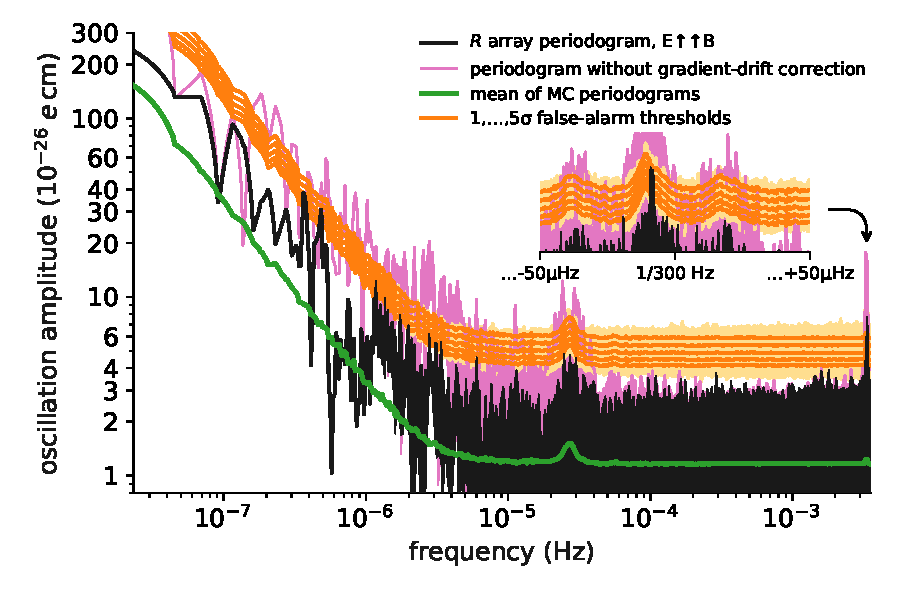
\includegraphics[width=\linewidth]{gfx/axions/detection_psi_inset_gc.pdf}
  \caption{Periodogram of the $R$ time series of the PSI experiment data, sensitive to oscillations in the quantity $d_\mathrm{n} - \left( \mu_\mathrm{n} / \mu_\mathrm{Hg} \right) \, d_\mathrm{Hg}$, taken with the $\boldsymbol{E}$ and $\boldsymbol{B}$ fields parallel (black line).
  The mean of MC-generated periodograms, assuming no signal, is depicted in green. MC is used to calculate $1,2,…,5\,\sigma$ false-alarm thresholds, depicted in light orange.
  For clarity, we also plot the smoothed version in orange.
  There are two regions where a rise in the amplitude is expected, namely around \SI{28}{\micro\hertz} (inverse of 10 hours) and \SI{3.3}{\milli\hertz} (inverse of 300 seconds), due to the time structure of the data taking (see the main text for more details). The periodogram of non-gradient-drift-corrected data is shown in pink.}\label{fig:axions_PSI_detection}
\end{figure}

The LSSA periodogram of the $E \uparrow \uparrow B$ subset is presented in Fig.\,\ref{fig:axions_PSI_detection} in black. The average null-hypothesis periodogram is depicted in green and the false-alarm thresholds in orange. An inset details the region around inverse \SI{300}{\second}, the cycle frequency.
There are two regions of expected rise in the oscillation amplitude due to the time structure of the data collection.
\marginpar{Recall the discussion in Sec.\,\ref{sec:a_null_hypothesis_test} about the peaks in the periodogram solely due to the time structure of the series.}
The one around \SI{28}{\micro\hertz} (the inverse of 10 hours) corresponds to the period of the reversal of the electric field. Each ramp caused a small break in the data taking (one cycle was missed).
The other, around \SI{3.3}{\milli\hertz}, the inverse of \SI{300}{\second}, corresponds to the cycle repetition rate.

The periodogram of the $R$ time series without the gradient-drift correction is shown in pink in Fig.\,\ref{fig:axions_PSI_detection}.
The correction had an effect only for frequencies slower than the period of the reversal of the electric field and around the narrow window around inverse \SI{300}{\second}.
It should be pointed out, that \SI{300}{\second} is the approximate sampling period and as such it is likely to have some of the high power observed in low frequencies folded onto it (see the reasoning in Ref.\,\cite{Shannon1949}).
The period of the electric field change had been deliberately chosen such, that was possibly infrequent, but still occurring when the magnetic field had not drifted significantly away.

In the periodogram of the gradient-corrected time series there are five
trial frequencies for which the $3\upsigma$ false-alarm threshold is exceeded,
two of which, including the largest excess with a $6\upsigma$ significance, occur in a \SI{100}{\micro\hertz} region around the inverse of \SI{300}{\second}, while the other three are in the low-frequency region, longer than an inverse length of a sequence.
 The periodograms for the other two datasets, very similar to this one, can be found in App.\,\ref{ch:alp_appendix}.
In the other sensitive set there are three excesses above the $3\upsigma$ threshold (the highest is $5\upsigma$), all constrained to the same two regions. In the control dataset, only the $1\upsigma$ threshold is exceeded. None of the excesses fulfill the detection criteria, in particular the requirement to be present in both $E \uparrow \uparrow B$ and $E \uparrow \downarrow B$ periodograms with opposite phases.

\begin{figure}
  \centering
  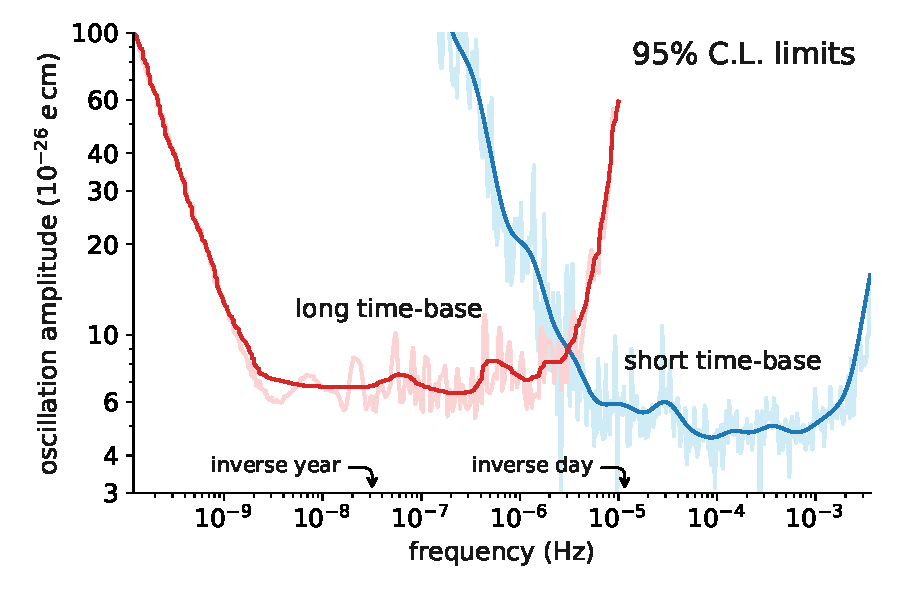
\includegraphics[width=\linewidth]{gfx/axions/psi_ill_1e-26ecm.pdf}
  \caption{Limits on the amplitude of oscillation in the quantity $d_\text{n} - \frac{\mu_\text{n}}{\mu_\text{Hg}} \, d_\text{Hg}$, as a function of frequency thereof. The are above the curves is excluded on the \SI{95}{\percent}~C.L.
  The limit of this analysis (of the PSI data) are depicted in blue; the red curve depicts the limits of the complementary analysis of the ILL-based experiment's data~\cite{AyresThesis,PhysRevX.7.041034}.
  The numerically obtained limits are depicted with faint lines; the bold lines are smoothed.}
\label{fig:axions_limits_nEDM}
\end{figure}

As no significant signals have been observed, limits could be placed to exclude the observations that would have been detected.
The limits, obtained numerically in a way discussed in Sec.\,\ref{sec:signal_hypotheses_tests}, are depicted in Fig.\,\ref{fig:axions_limits_nEDM} in blue (labelled ``short time-base'').
This analysis was most sensitive for periods between the duration of a sequence, around two days, and cycle repetition, \SI{300}{\second}.
Amplitudes down to \SI{5e-26}{\elementarycharge\centi\meter} could be excluded on the \SI{95}{\percent}~C.L.
The limits of the long time-base analysis, the one of the ILL-based experiment's data~\cite{AyresThesis,PhysRevX.7.041034}, are depicted in red.
Complementarily, they are sensitive to periods just below the duration of a sequence and go down to about a decade.

\begin{figure}
  \centering
  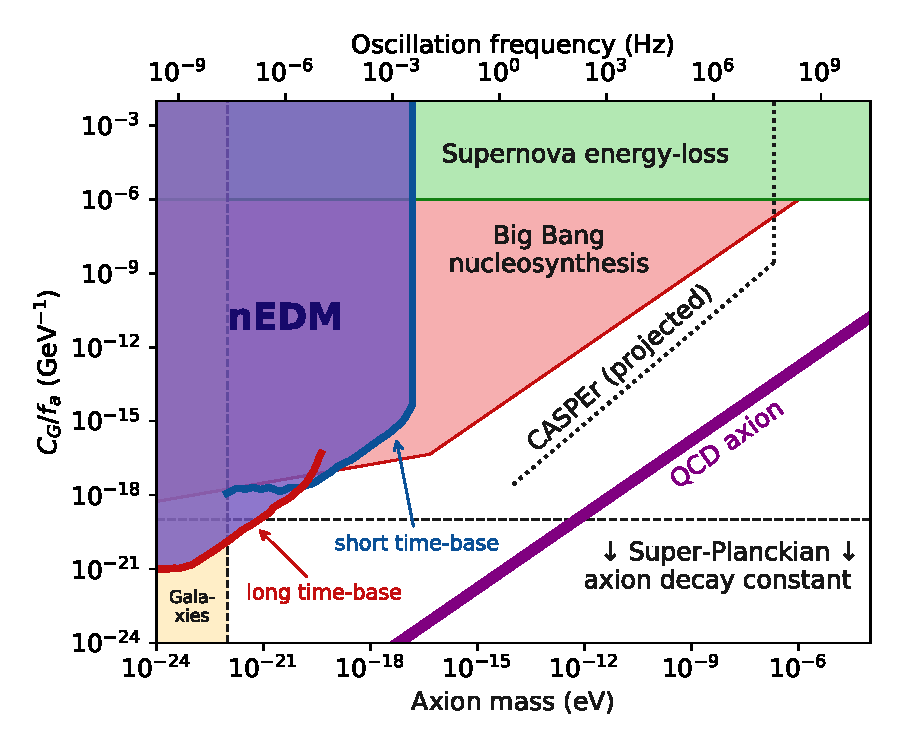
\includegraphics[width=\linewidth]{gfx/axions/psi_ill_axion_limits_v7.pdf}
  \caption{Limits on the interaction of an axion with the gluons (\SI{95}{\percent}~C.L.).
  The parameter space is spanned by the axion's mass (horizontal) and the strength of the coupling (vertical).
  It has been assumed that axions saturate the local cold dark matter density.
  Other depicted constraints are: Big Bang nucleosynthesis (red, \SI{95}{\percent}~C.L.)~\cite{Blum2014,StadnikThesis,Stadnik2015D}; supernova energy-loss bounds (green, order of magnitude)~\cite{Graham2013,Raffelt1990Review,Raffelt2008LNP} and consistency with observations of galaxies (orange)~\cite{Marsh2015Review,Marsh2015B,Schive2015,Marsh2017}.
  The projected reach of the proposed CASPEr experiment is depicted with a dotted black line~\cite{CASPEr2014}, and the parameter space for the canonical QCD axion with a purple band.}
\label{fig:axions_limits_coupling}
\end{figure}

The oscillating-nEDM limits were interpreted as limits on the axion-gluon coupling (following the Eq.\,\ref{eq:nEDM_axion}).
The results are presented in the axion space, spanned by their mass and the strength of the coupling, in Fig.\,\ref{fig:axions_limits_coupling}.
The limits are presented in the landscape of already existing cosmological limits: axions with a mass below \SI{e-22}{\electronvolt} have their Compton wavelength larger than the size of the smallest dwarf galaxies and, therefore, could not be the sole constituent of dark matter~\cite{Marsh2015Review}; the influence of axions in the red-shaded area on the Big Bang nucleosynthesis would result in an underproduction of ${}^4$He~\cite{Blum2014}; the green area was excluded based on the observations of the supernova SN1987A, where excess cooling by axion emission would have been observed~\cite{Graham2013}.
The limits are not only the first laboratory constraints on the axion-gluon coupling, but also improve on the existing cosmological exclusions.




\section{Axion-Wind analysis}
The analysis described so far was concerned with the scalar coupling of the axions to gluons, which looks like an oscillation in the electric dipole moment of the neutron.
The same data set, and the same analysis techniques, were also used for a different coupling---a derivative one of axions to nucleons. This coupling acts like an additional dynamic magnetic field. The data were split based on the direction of the holding magnetic field $B_0$, as indicated in Fig.\,\ref{fig:axions_wind_time_domain}. The axion-wind coupling is insensitive to the electric field in the experiment.

\begin{figure}
  \centering
  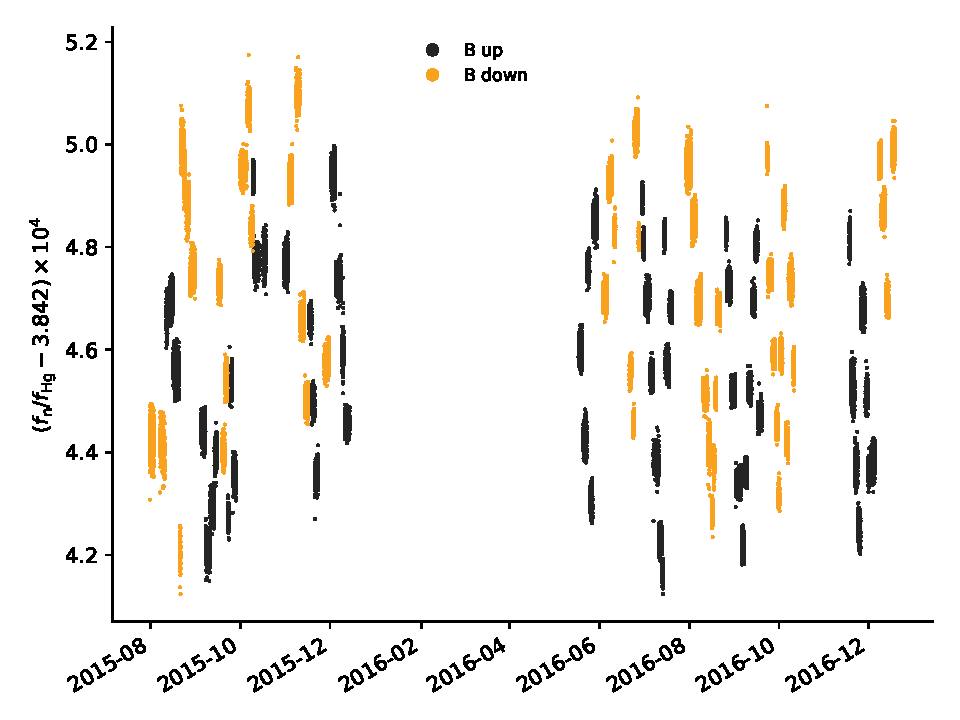
\includegraphics[width=\linewidth]{gfx/axions/wind_winddeltah4mm_time_domain_inset_no_yerr.pdf}
  \caption{The $R$ time series measured at PSI measured between July 2015 and December 2016 with the orientation of the magnetic field marked. The two orientations form the two datasets for the axion-wind analysis.}\label{fig:axions_wind_time_domain}
\end{figure}

The induced energy level shift, Eq.\,\ref{potential_axion-wind}, is proportional to the projection of experiment's quantisation axis on the momentum of the axions.
Because the latter arises due to the Earth's traversing the galactic axion field in the Solar System's movement around the Milky Way's centre, the effect is called the axion-wind~\cite{Stadnik2014A}.
The Earth additionally spins, causing the effect to be modulated with the sidereal frequency $\Omega_\text{sid}$, equal to \num[detect-all=true]{23.9344699} hours. \note{ref needed}
\marginpar{The sidereal frequency is the one of the Earth's spinning as seen in the reference of distant stars.}
The modulation would have produced a triplet of lines as a signal in the periodogram.
The highest peak would be at the frequency of the oscillation of the axion field, and would be accompanied by two additional ones on either side, $\Omega_\text{sid}$ away from it.

There were two datasets, with the magnetic field pointing in either way along gravity, both sensitive to the effect.
The periodograms can be found in App.\note{reference them}.
There are 44 frequencies with power above the 3$\upsigma$ threshold in $B\uparrow$ and 36 in $B\downarrow$.
Ony for two frequencies the threshold is exceeded in both data sets simultaneously: \SI{3.42969}{\micro\hertz} and \SI{3.32568}{\milli\hertz}.
Neither  fulfilled the requirement of the phase being opposite in the two data sets.

The lack of a statistically significant signal compatible with the axion model allowed us to put limits on the axion-nucleon coupling, depicted in Fig.\,\ref{fig:axions_wind_limits}. The limits improves upon the existing laboratory constraints by a factor of 40.

\begin{figure}
  \centering
  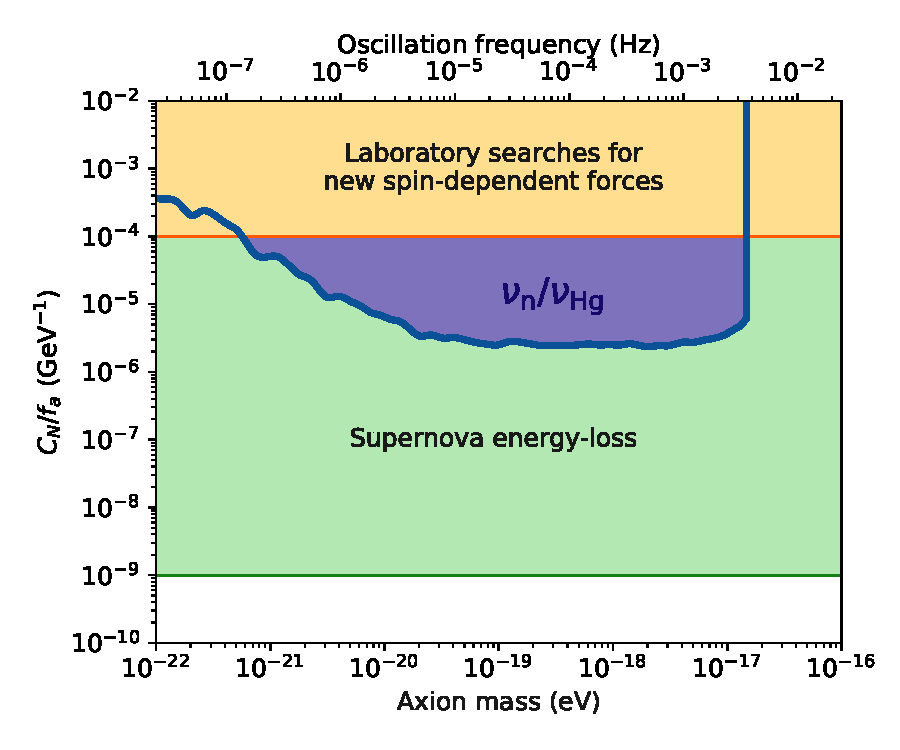
\includegraphics[width=\linewidth]{gfx/axions/psi_ill_axion_wind_limits_v1.pdf}
  \caption{Excluded regions of the space of the coupling of axions to nucleons (Eq.\,\ref{potential_axion-wind}). The green region is excluded from observations of the SN1987A supernova~\cite{PhysRevX.7.041034}, and the yellow one from K--${}^3$He magnetometry~\cite{Romalis2009_NF}. The blue region, is the exclusion arising from this analysis.}\label{fig:axions_wind_limits}
\end{figure}




\section{Outlook}
There are three directions in which the nEDM-based axion dark matter search could continue.
In order to improve sensitivity vertically, to be sensitive to more weekly coupled or less abundant axions, the overall sensitivity of the nEDM measurement would need to be improved.
Following Eq.\,\ref{eq:nEDM_sensitivity} it would require more neutrons, a higher electric field or a longer spin-precession time.
% \marginpar{In Eq\,\ref{eq:nEDM_sensitivity} $\alpha$ is already \ldots, precession time $T$ can only be improved so long---it is fundamentally limited by the neutron life-time (give the number.)}
The global community already spares no effort in this respect.

The second way would be to improve sensitivity for slower oscillations, that is  lighter axions.
It was limited by the span of the data set---four years in the case of the ILL nEDM data set.
Combining the ILL and PSI data into one time series would increase it to 19 years.
It could not yet be done at the time for two reasons.
Firstly, the PSI data were still blinded.
Secondly, the static nEDM analysis, which would produce per-sequence nEDM estimates, was still ongoing.
In any case, axions oscillating this slow would be so light, that their Compton wavelength would not fit in small dwarf galaxies~\cite{Marsh2015Review}, which rules them out as the sole dark matter constituent.

The third direction would be the high-frequency, heavy-axions one.
It was limited by the sampling frequency of the system, the cycle repetition rate.
% \marginpar{At PSI the cycles were synchronised to the pulses of a kicker magnet, which redirected a proton beam onto the target of the UCN source.}
The measurements could be conducted with a shorter cycle time.
This would, however, worsen the sensitivity, as the loss in Eq.\,\ref{eq:nEDM_sensitivity} is linear, and the gain from the improved statistics scales with the square root.
A repetition period faster than \SI{10}{\second} is hard to imagine.
A real improvement in this direction would require changing the principle of the measurement.




\section{Resonant oscillating nEDM search}
The periodogram-based searches for Dark Matter were sensitive to a wide range of frequencies.
In contrast resonant searches (for example ADMX~\cite{PhysRevLett.104.041301}, or the proposed CASPEr~\cite{CASPEr2014}) are sensitive at a any given time only to a relatively narrow band of frequencies.
Covering a wide range requires scanning.
In this section a resonant search of an oscillating nEDM is proposed, which would give access to faster oscillations than the periodogram-based method.

% Many of the axion searches are resonant based.~\cite{PhysRevLett.104.041301,CASPEr2014} \note{some references}.
% The standard instrument to look for an axion-photon coupling, called a haloscope \note{verity}, consists of ultra-low-noise resonant cavity, where axions can produce photons, detected with an antenna \note{is it an antenna?}.
% At any given time the measurement is sensitive only to a narrow band of photon energies (or frequencies), the width given by the finesse \note{verity} of the cavity. To cover a wide range the tuning of the cavity is scanned. In this section an idea of a resonant oscillating nEDM search is pursued.

For polarised neutrons in a magnetic field a transverse oscillating coupling induces a coherent Rabi oscillation between the spin-up and spin-down states.
For example, a Ramsey cycle begins with a $\uppi/2$ flip induced by an oscillating transverse magnetic field, its frequency tuned to the Larmor one and its length tuned such, that the Rabi oscillation stops when the polarisation is in the transverse plane. Should the nEDM oscillate, an oscillating transverse coupling could be realised with a static magnetic field \emph{perpendicular} to the holding magnetic field $\mathbf{B}$. Then, when the frequency of the nEDM oscillation is tuned to the Larmor one, the neutrons would undergo a Rabi nutation, which could be detected. Scanning the magnetic field in the range \SIrange[range-phrase=--]{0.1}{10}{\micro\tesla} would cover frequencies \SIrange[range-phrase=--]{3}{300}{\hertz}.

\begin{figure}
  \centering
  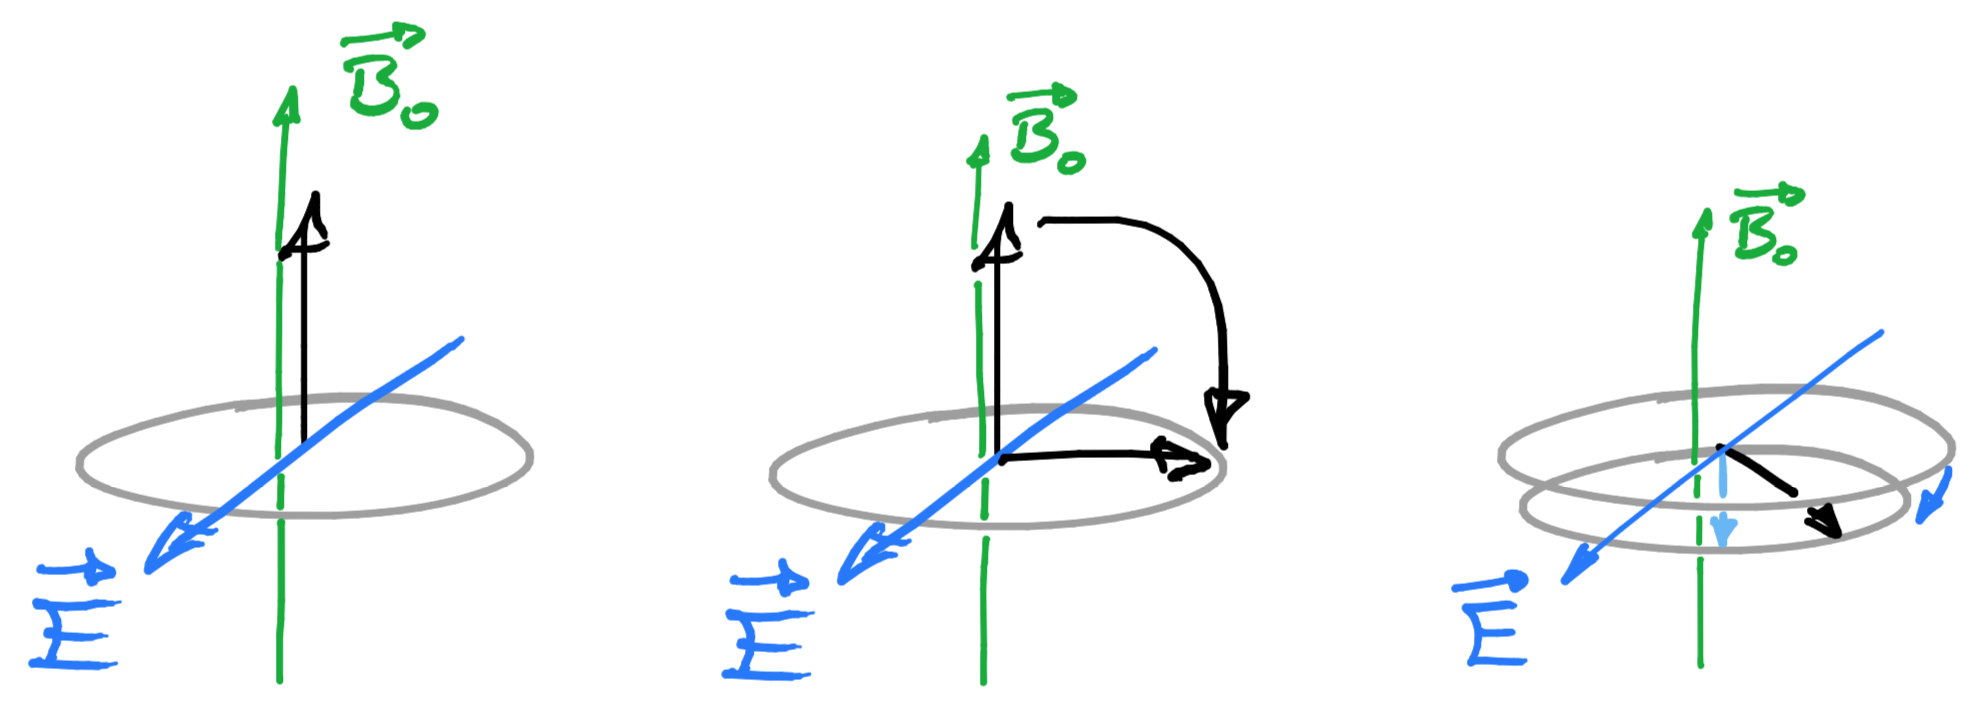
\includegraphics[width=\linewidth]{gfx/axions/resonant_effect.png}
  \caption{The behaviour of the spin population in a resonant oscillating EDM search.
  One starts with an ensemble polarised along the holding magnetic field $B_0$.
  The electric field is perpendicular.
  Then, the polarisation is flipped by $\pi$/2 and Larmor precession starts.
  The combination of the electric field and an oscillating EDM would induce a Rabi nutation.
  The direction of the nutation is determined by the relative phase of the Larmor precession and the EDM oscillation.}\label{fig:axions_resonant_effect}
\end{figure}

In the proposed scheme, sketched in Fig.\,\ref{fig:axions_resonant_effect}, the neutrons start polarised along the holding field and are put into the Larmor precession with a $\uppi/2$ flip. The oscillating nEDM would then induce a Rabi nutation and a net polarisation along the $\mathbf{B}$ direction would build up. This net polarisation could be measured. The direction of the nutation depends on the phase difference between the Larmor precession (defined by the phase of the $\uppi/2$ pulse) and the oscillating nEDM\@.

In order to estimate the sensitivity of such a search consider the Hamiltonian for a neutron in a magnetic field
\begin{equation}
  H = - \boldsymbol{\upmu}_\text{n} \cdot \mathbf{B} = - \gamma_\text{n} \mathbf{S} \cdot \mathbf{B}
\end{equation}
for which the Larmor frequency is
\begin{equation}
  \omega_0 = \frac{\mu_\text{n} B}{S} = \frac{2 \mu_\text{n} B}{\hbar} = \gamma_\text{n} B \ .
\end{equation}
In the presence of an electric field perpendicular to $\mathbf{B}$ a harmonically oscillating nEDM adds an additional term to the Hamiltonian
\begin{equation}
  H = - \gamma_\text{n} \mathbf{B} \cdot \mathbf{S} - \mathbf{d}_\text{n}^0 \sin (\omega_0 t) \cdot \mathbf{E} \ ,
\end{equation}
where we assume the Larmor frequency to be resonant with the oscillating nEDM, and a phase difference of \ang{90} between the spin's precession and the nEDM oscillation.
The Hamiltonian is the same when nEDM is static and the term $\sin (\omega_0 t)$ comes from an oscillating electric field $\mathbf{E}$. The oscillating field can be decomposed into two fields rotating in the opposite directions, each with the amplitude $E/2$. In a rotating frame spinning around $\mathbf{B}$ with the frequency $\omega_0$ the field $\mathbf{B}$ vanishes. The $\mathbf{E}$ component which rotates with the spin is static~\cite{RamseyBook}:
\begin{equation}
  H_\text{rot} = d_\text{n}^{\,0} \, \frac{\mathbf{E}}{2} \cdot \mathbf{S} \ ,
\end{equation}
whereas the other spin with frequency $2 \omega_0$ and can be, in the first approximation, neglected~\cite{RamseyBook}.
In the rotating frame the spin precesses with the frequency
\begin{equation}
  \omega_\text{nut.} = \frac{d_\text{n}^{\,0} E }{2 \hbar} \ .
\end{equation}
After time $T$ the accumulated angle is
\begin{equation}
  \theta = \omega_\text{nut.} T = \frac{d_\text{n}^0 E }{2 \hbar} \, T \ .
  \label{eq:resonant_the_angle}
\end{equation}
At the end of the measurement the neutrons pass a spin analyser, which projects their polarisation on the axis of $\mathbf{B}$.
For $N_0$ neutrons the resonance curve has a shape
\begin{equation}
  N_{\uparrow \downarrow}(\theta) = \frac{N_0}{2} \left( 1 \pm \alpha \sin \theta  \right)  \ ,
\end{equation}
where $\alpha$ is the visibility parameter and the sign depends on which spin state is counted.
A change in the neutron counts for a small angle $\delta \theta$ is:
\begin{equation}
  \delta N = \frac{N_0}{2} \alpha \, \delta \theta \ .
  \label{eq:resonant_deltaN}
\end{equation}
Finally, the sensitivity is obtained from Eqs.\,\ref{eq:resonant_the_angle} and~\ref{eq:resonant_deltaN}, assuming it is dominated by the counting statistics $\sqrt{N_0/2}$
\begin{equation}
  \sigma_{d_n^{\,0}} = \frac{2 \hbar}{\sqrt{N_0/2} \alpha T E} \ .
\end{equation}
When both spin states are counted the sensitivity increases by a factor $\sqrt{2}$:
\begin{equation}
  \sigma_{d_n^{\,0}} = \frac{2 \hbar}{\sqrt{N_0} \alpha T E} \ .
\end{equation}

A \ang{90} phase difference between the nEDM oscillation and spin precession (defined by the phase of the $\uppi/2$ pulse) is assumed.
On average an additional factor of $\sqrt{2}$ is lost due to the non-matching phases.
Doing two measurements with the phases of the $\pi/2$ pulses shifted by \ang{90}, one having a sine-like sensitivity other a cosine-like, gives a flat sensitivity for all phases of the nEDM oscillation.

\begin{figure}
  \centering
  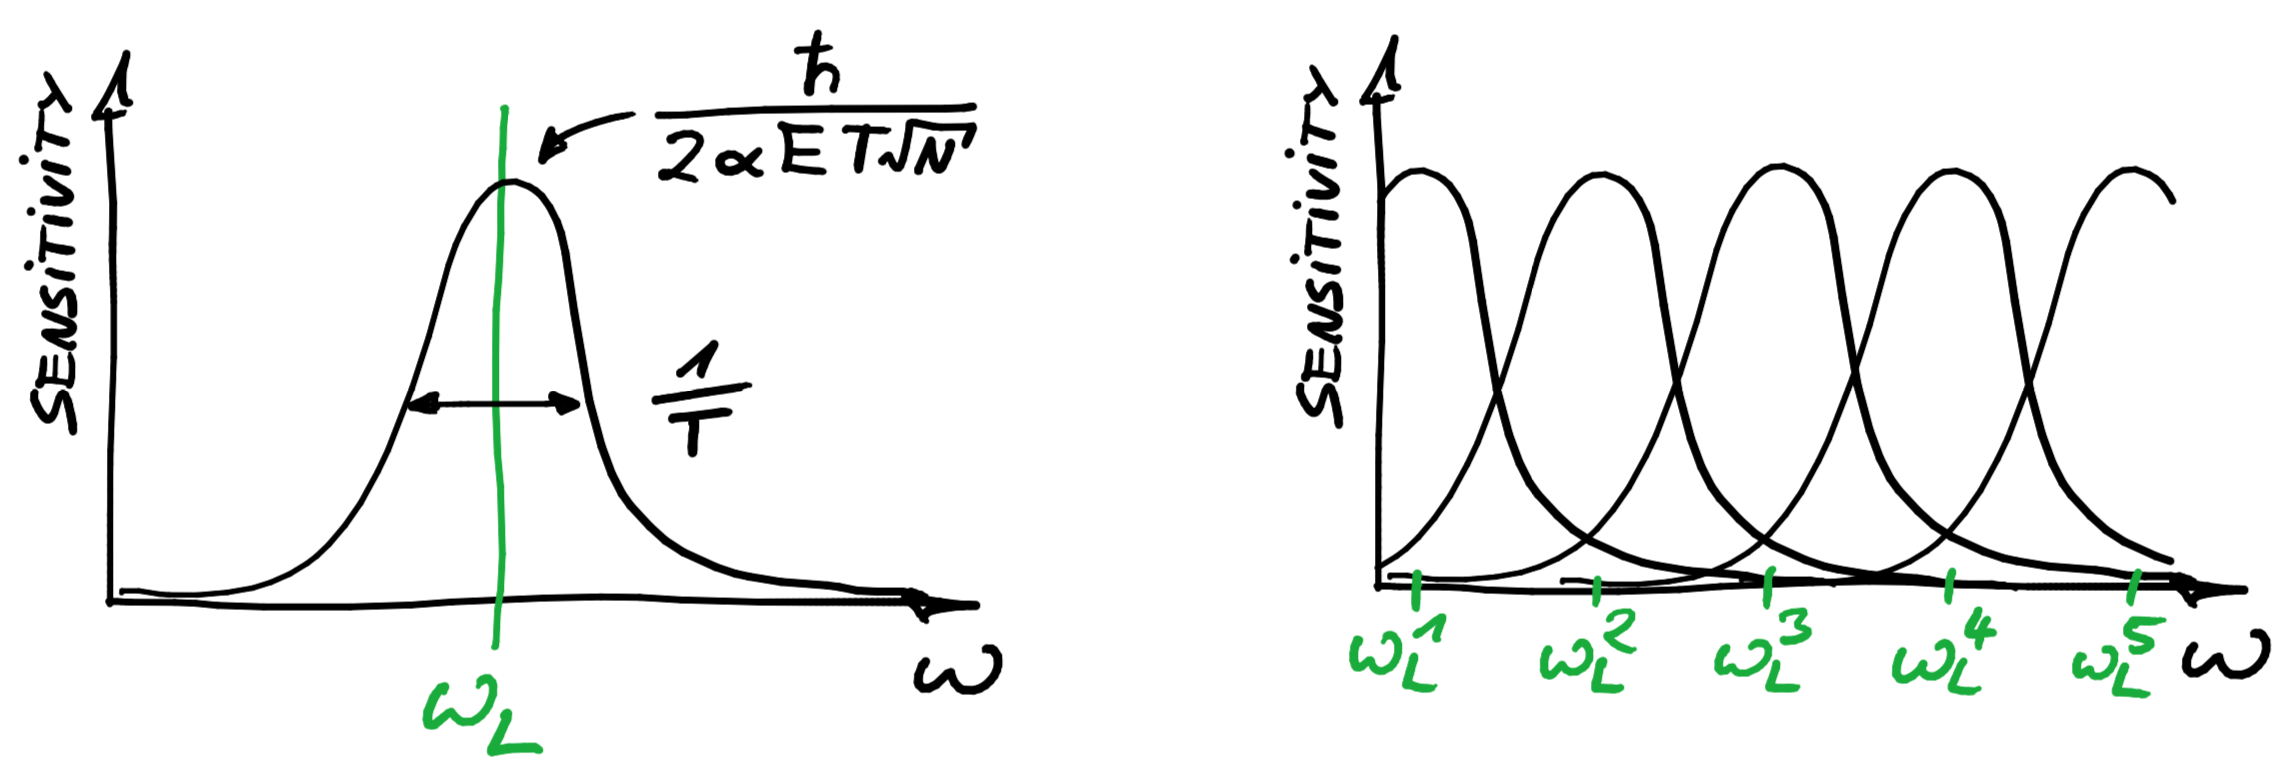
\includegraphics[width=\linewidth]{gfx/axions/resonant_sensitivity.png}
  \caption{\emph{Left:} the sensitivity of the resonant search has a width equal to the inverse interaction time.
  \emph{Right:} a broad-band sensitivity needs to be built up with multiple measurements.}\label{fig:axions_resonant_sensitivity}
\end{figure}

The search is resonant---at any given time the full sensitivity is achieved only for the nEDM oscillation frequency equal to the Larmor one.
To cover a wide spectrum the strength of the magnetic field $\mathbf{B}$ would need to be scanned.
The width of the sensitivity peak is $1/T$; the broad-band search would need to be built up from many of those, as depicted in Fig.\,\ref{fig:axions_resonant_sensitivity}.

In order to perform a \SIrange[range-phrase=--]{3}{300}{\hertz} scan in 1000 cycles (3 days of operation of the n2EDM experiment at PSI) the width of the resonance would need to be
\begin{equation}
  T = {\left( \frac{1}{1000} \left( \SI{300}{\hertz} - \SI{3}{\hertz} \right)  \right)}^{-1} \approx \SI{3}{\second} \ .
\end{equation}
With the baseline parameters of the n2EDM experiment at PSI, $\alpha = 0.8$, $E = \SI{15}{\kilo\volt\per\centi\metre}$, $N_0 = \num{121000}$, the per-cycle sensitivity would be 
\begin{equation}
  \sigma_{d_n} = \SI{1e-22}{\elementarycharge\centi\metre} \ .
\end{equation}
The region of an axion coupling to gluons that could be excluded is depicted in Fig.\,\ref{fig:axions_prediction}.

\begin{figure}
  \centering
  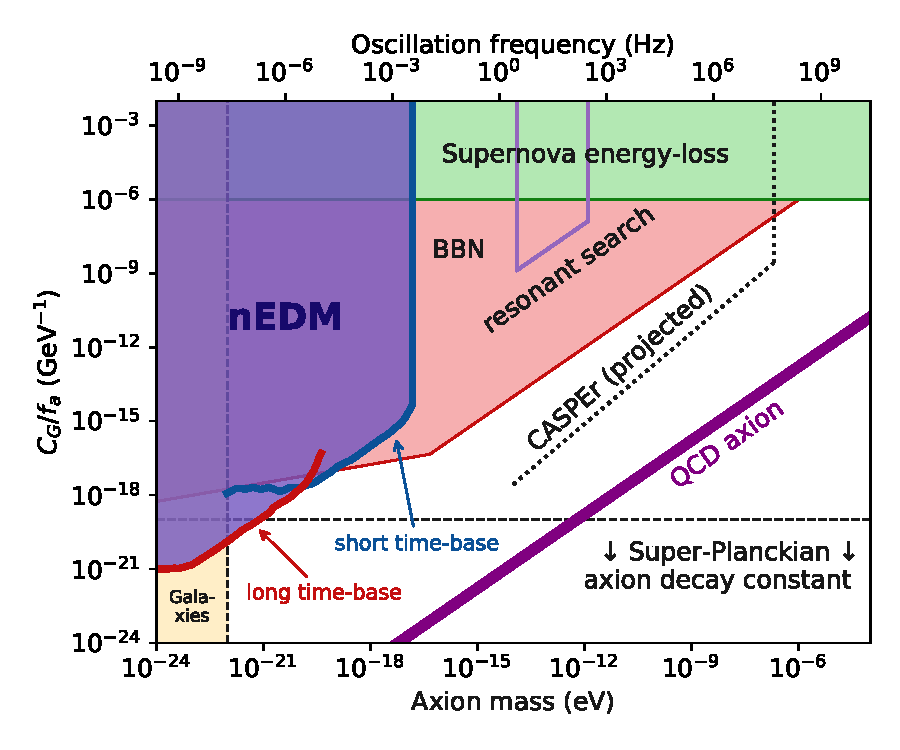
\includegraphics[width=\linewidth]{gfx/axions/resonant_search_exclusion_1000cycles_n2EDM.pdf}
  \caption{Sensitivity prediction for a 1000 cycles long resonant oscillating nEDM search. A scan of the magnetic field in the range \SIrange[range-phrase=--]{0.1}{10}{\micro\tesla} gives the interaction time $T = \SI{3}{\second}$. The parameters of the baseline n2EDM design were used: $\alpha = 0.8$, $E = \SI{15}{\kilo\volt\per\centi\metre}$, $N_0 = \num{121000}$. See Fig.\,\ref{fig:axions_limits_coupling} for a detailed of the other limits.}\label{fig:axions_prediction}
\end{figure}

An important systematic effect would be the quality of the $\uppi/2$ pulse.
Polarisation remaining after it could be misinterpreted as a signal.
However, the effect scales linearly with the electric field $E$ and the interaction time $T$.
Both could be varied, in particular the electric field reversed, in a series of coherent measurements, which would need to be performed at each frequency.
The length of a series is limited by the coherence of the expected signal, \num{e6} in the case of an axion-induced nEDM oscillation.




\section*{Axion Analysis -- Conclusion}
Ultralight axion-like particles are compelling candidates for dark matter.
Besides interacting gravitationally they could couple to gluons and nucleons.
This coupling could be detected by the nEDM measurement at PSI\@.
Axions could induce harmonic oscillations in the time series of the ratio of the spin-precession frequencies of stored neutrons and ${}^{199}$Hg atoms.
The least squares spectral analysis was used to produce periodograms of the data measured at PSI\@.
The statistical treatment of the periodograms, largely based on Monte Carlo simulations, resulted in no significant signal.
The analysis of the electric-field correlated data gave the first laboratory constraints on the scalar coupling of axions to gluons and improved an astrophysical limits by up to three orders of magnitude.
The null result of the search in the magnetic-field correlated data improved the existing laboratory constraints by up to a factor of 40.